\documentclass[11pt]{article}
\usepackage[margin=1in]{geometry}
\usepackage{graphicx}
\usepackage{amsmath}
\usepackage{amssymb}
\usepackage{float}
\usepackage{subcaption}

\title{July 15, 2021 Meeting Agenda}

\begin{document}
\maketitle

\section{Judge Convex Hulls}
  I created the convex hulls using the actual sentence and the expected minimum sentence as calculated by Rhys Hester. The ones with the actual sentence are on the left column, and the ones with the expected minimum sentence are on the right column. I think the ones with the expected minimum sentence generally look better, some of the ones with the actual sentence have triangle shapes with most of the points on the bottom boundary and a single high point.

  \begin{figure}[H]
    \centering
    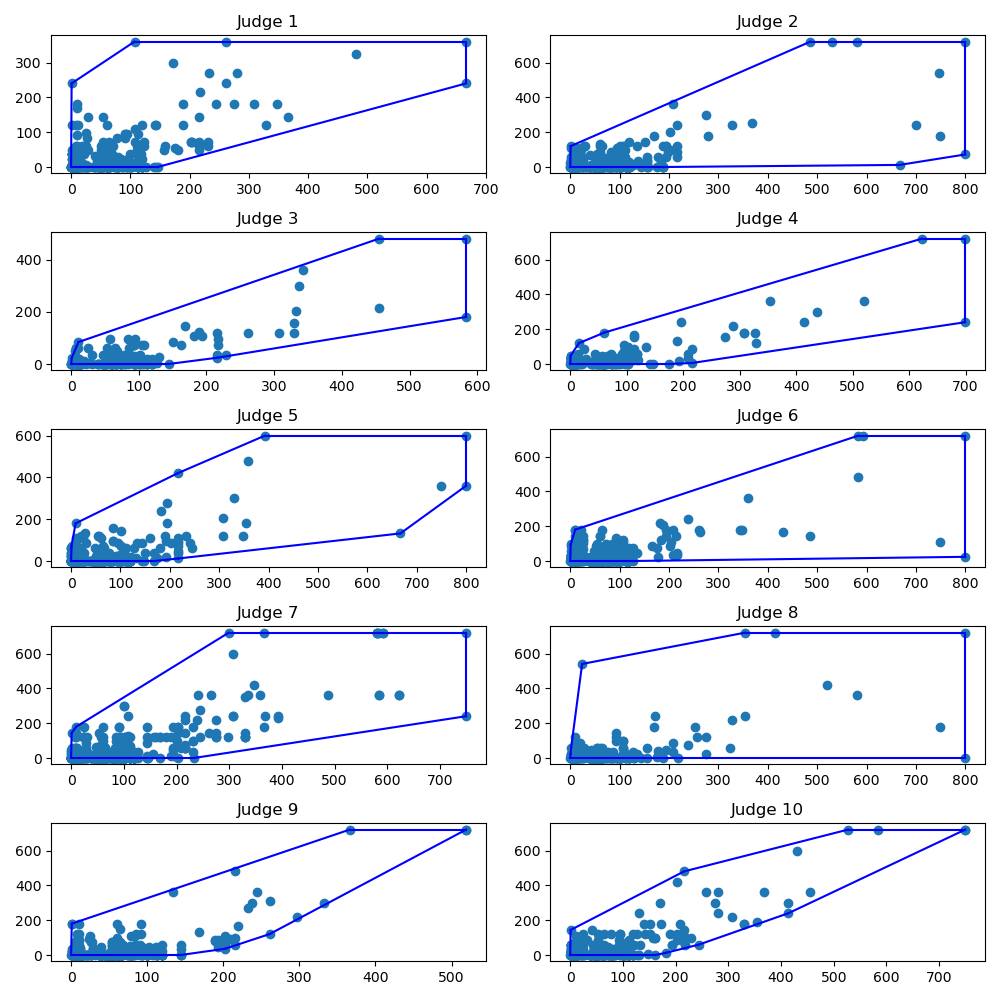
\includegraphics[width=0.9\textwidth]{../../../output/figures/Exploration/judge_convex_hulls_0.png}
  \end{figure}

  \begin{figure}[H]
    \centering
    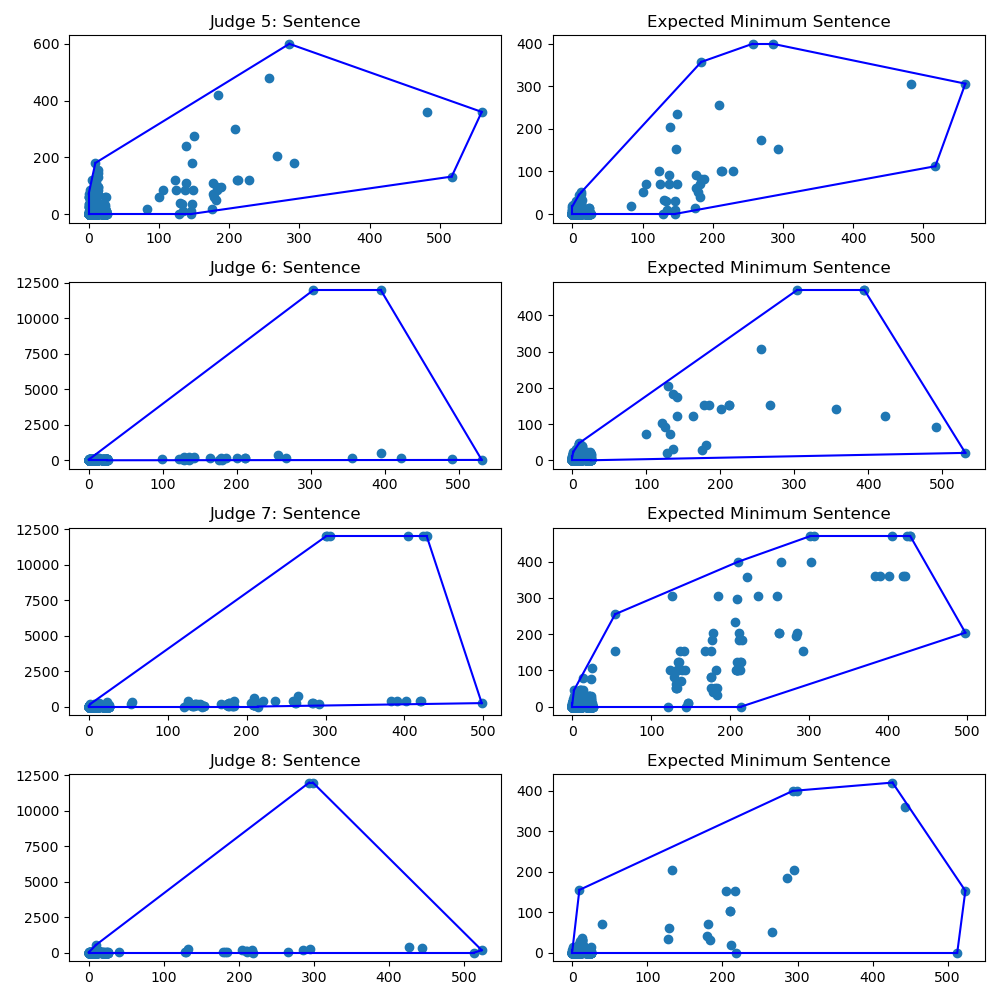
\includegraphics[width=0.9\textwidth]{../../../output/figures/Exploration/judge_convex_hulls_1.png}
  \end{figure}

  \begin{figure}[H]
    \centering
    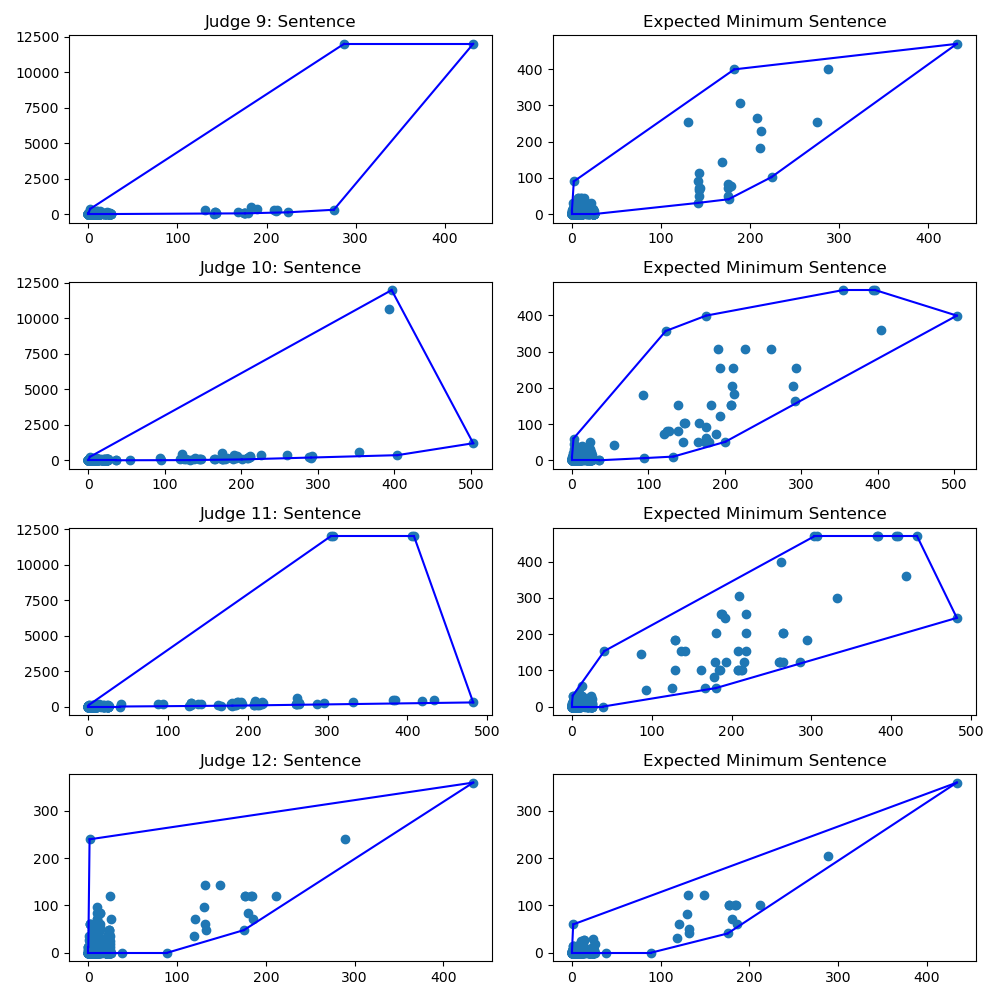
\includegraphics[width=0.9\textwidth]{../../../output/figures/Exploration/judge_convex_hulls_2.png}
  \end{figure}

  \begin{figure}[H]
    \centering
    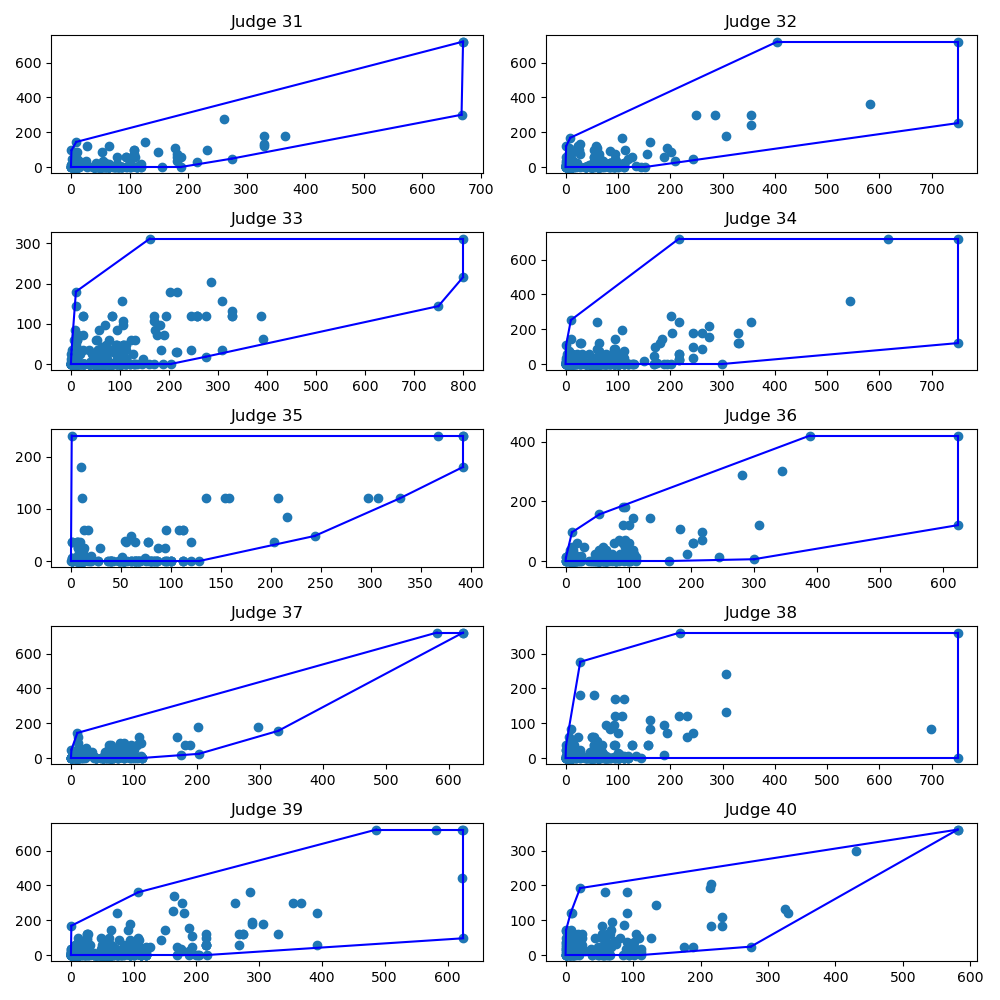
\includegraphics[width=0.9\textwidth]{../../../output/figures/Exploration/judge_convex_hulls_3.png}
  \end{figure}

  \begin{figure}[H]
    \centering
    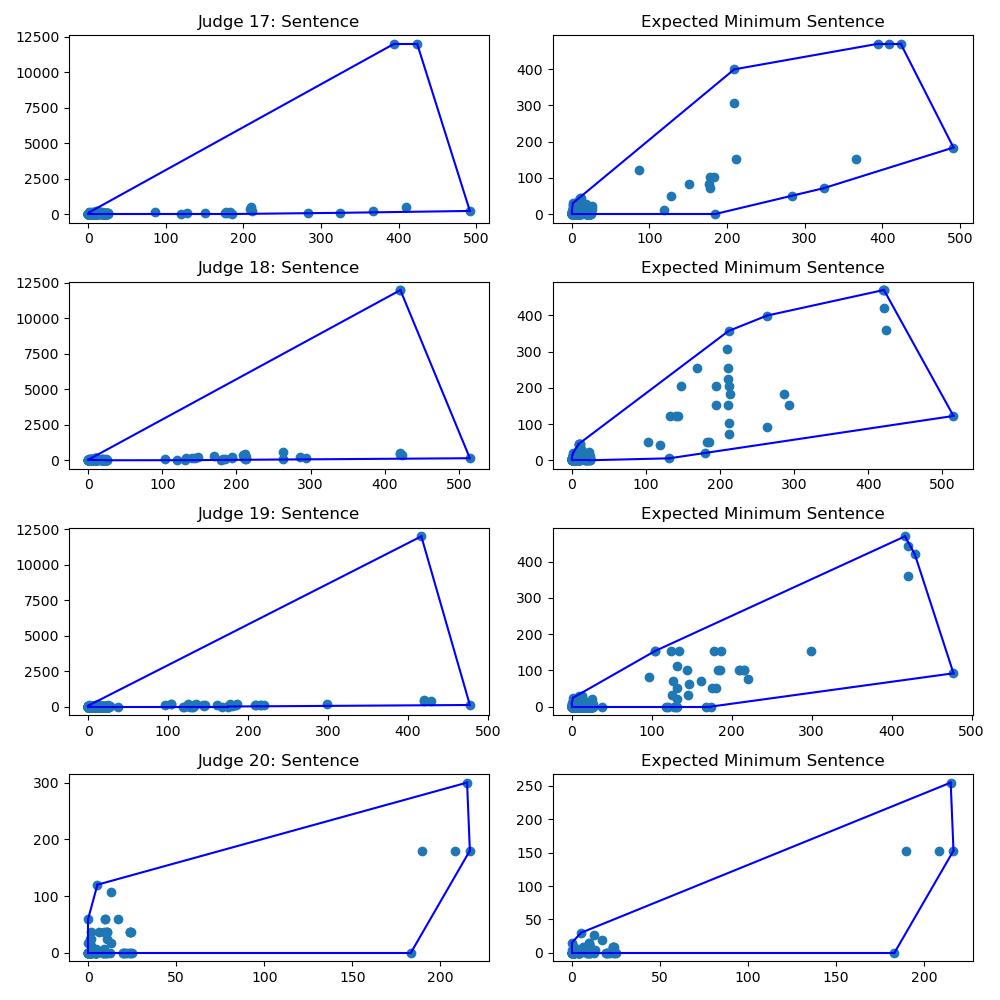
\includegraphics[width=0.9\textwidth]{../../../output/figures/Exploration/judge_convex_hulls_4.png}
  \end{figure}

  \begin{figure}[H]
    \centering
    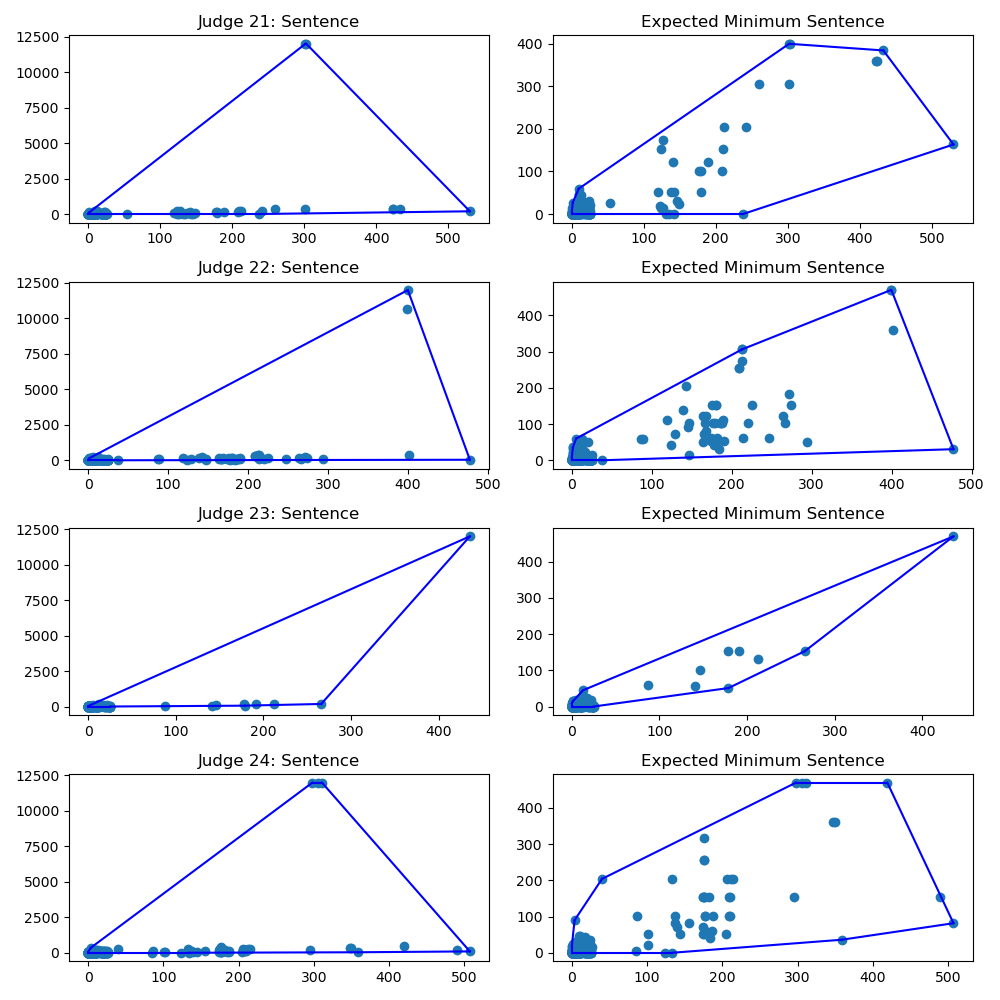
\includegraphics[width=0.9\textwidth]{../../../output/figures/Exploration/judge_convex_hulls_5.png}
  \end{figure}

  \begin{figure}[H]
    \centering
    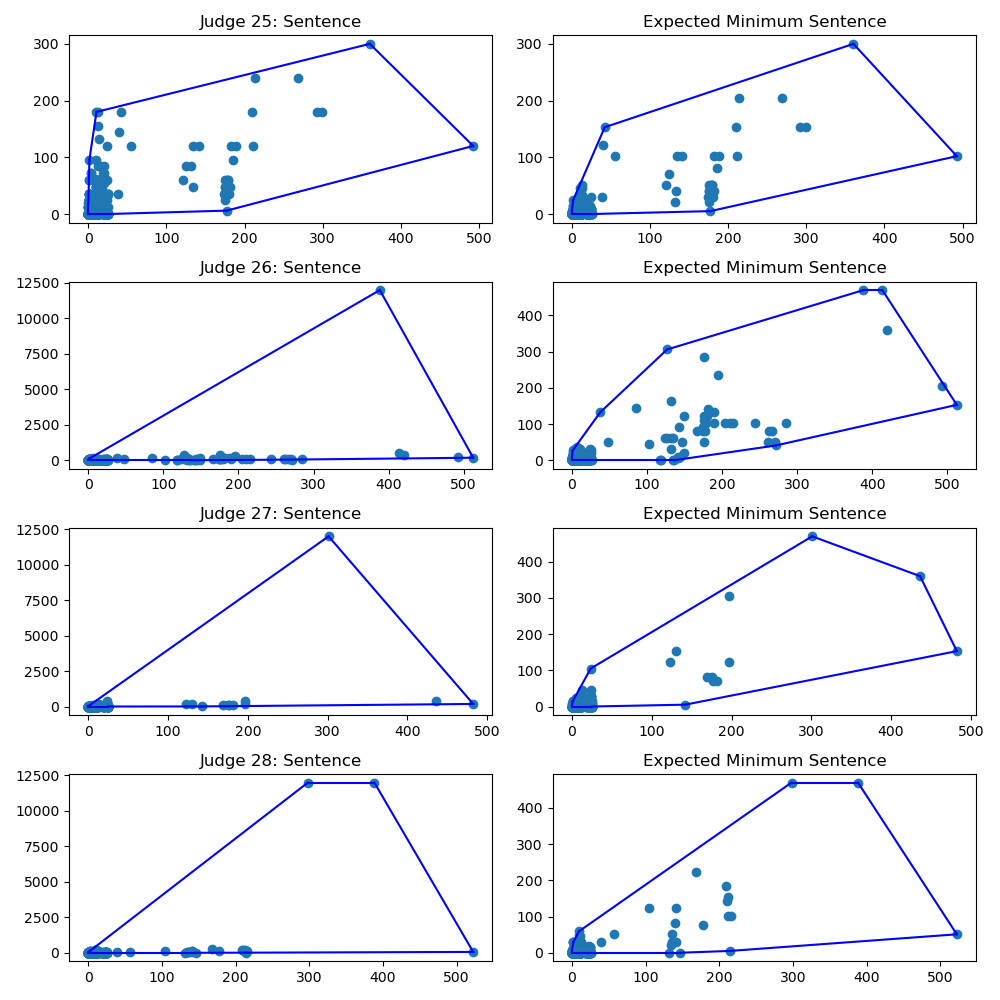
\includegraphics[width=0.9\textwidth]{../../../output/figures/Exploration/judge_convex_hulls_6.png}
  \end{figure}

  \begin{figure}[H]
    \centering
    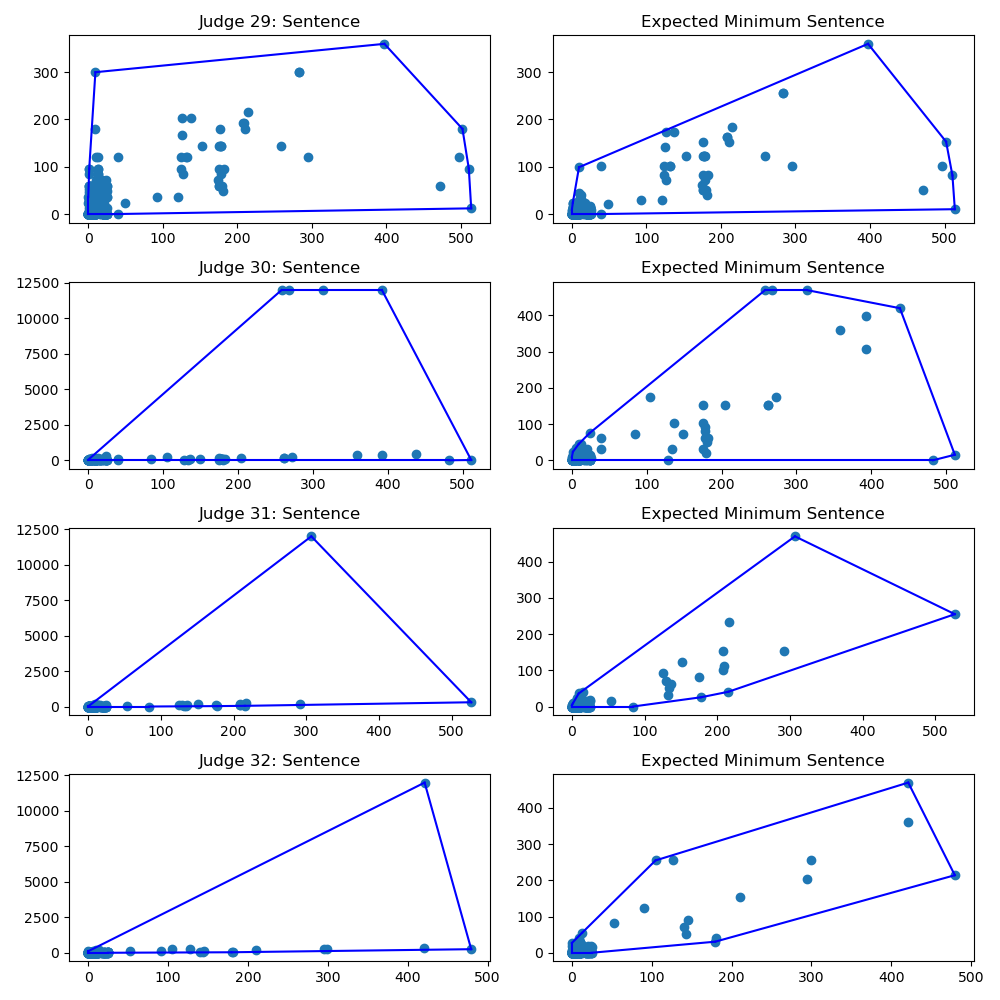
\includegraphics[width=0.9\textwidth]{../../../output/figures/Exploration/judge_convex_hulls_7.png}
  \end{figure}

  \begin{figure}[H]
    \centering
    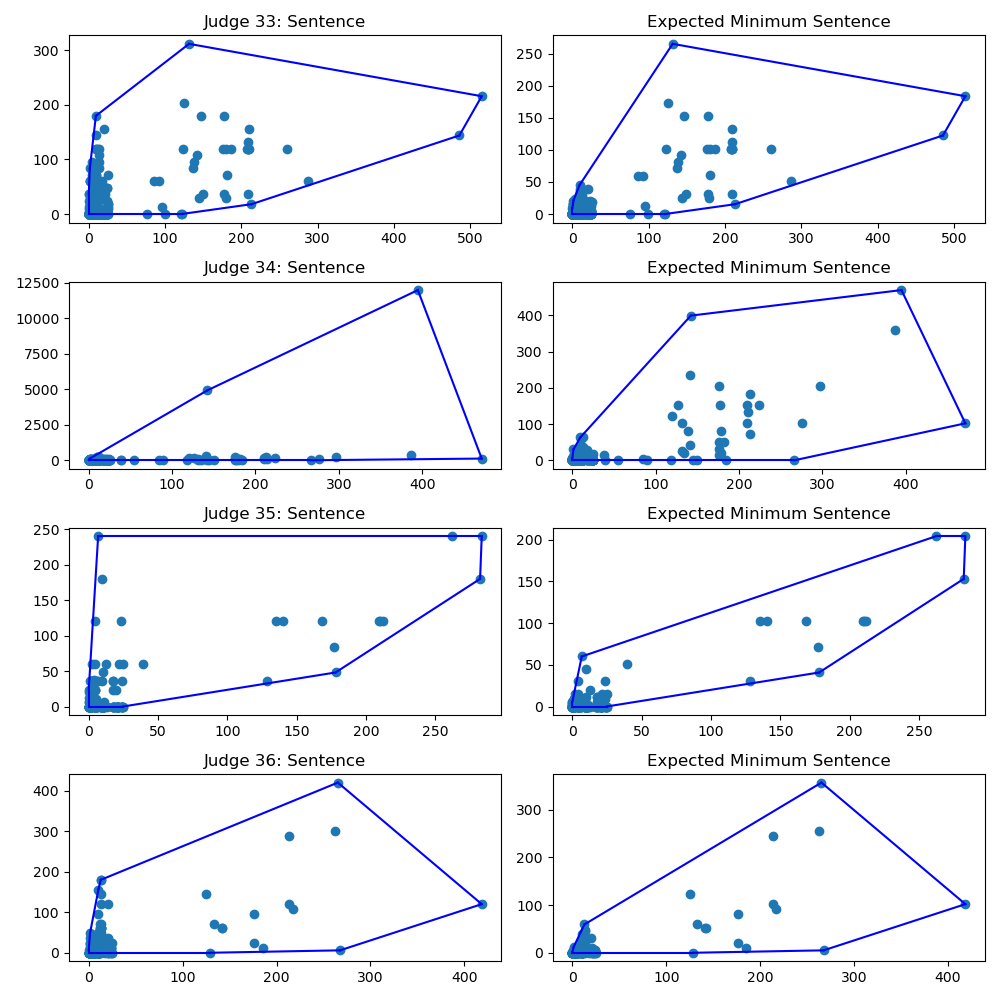
\includegraphics[width=0.9\textwidth]{../../../output/figures/Exploration/judge_convex_hulls_8.png}
  \end{figure}

  \begin{figure}[H]
    \centering
    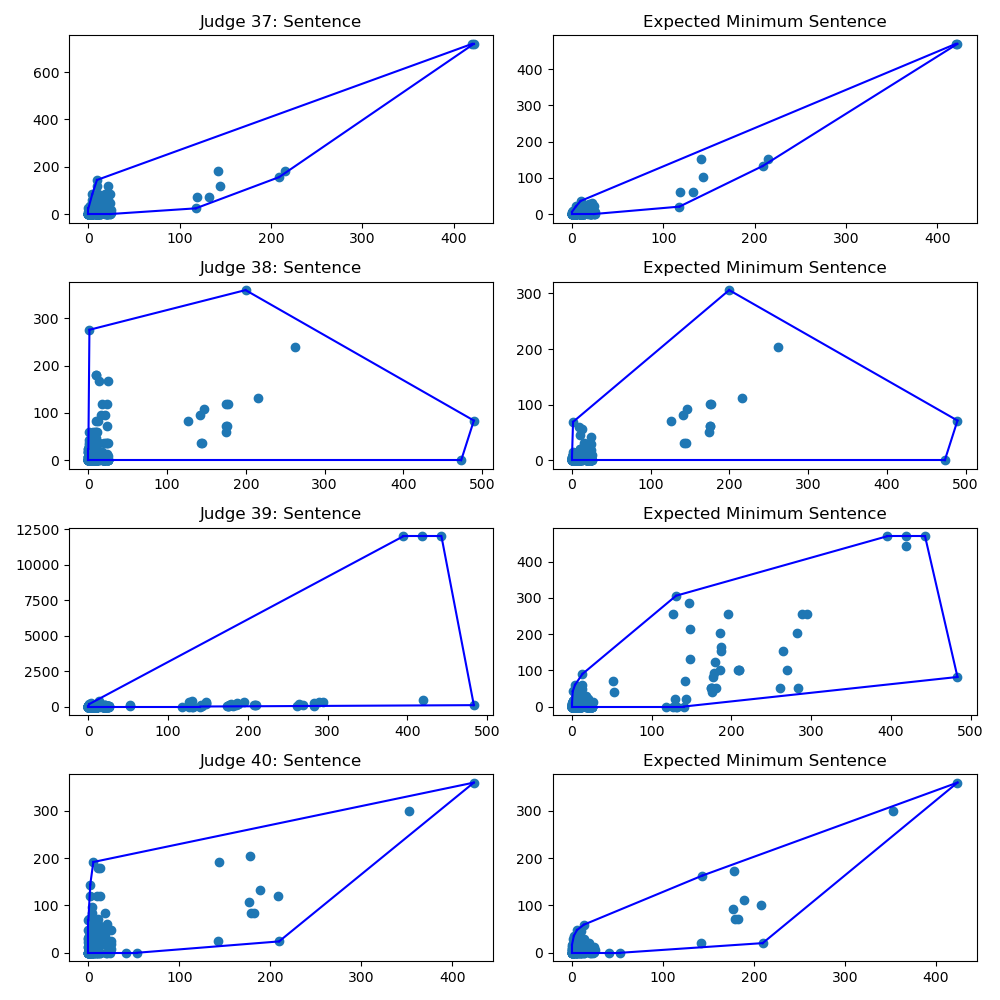
\includegraphics[width=0.9\textwidth]{../../../output/figures/Exploration/judge_convex_hulls_9.png}
  \end{figure}

  \begin{figure}[H]
    \centering
    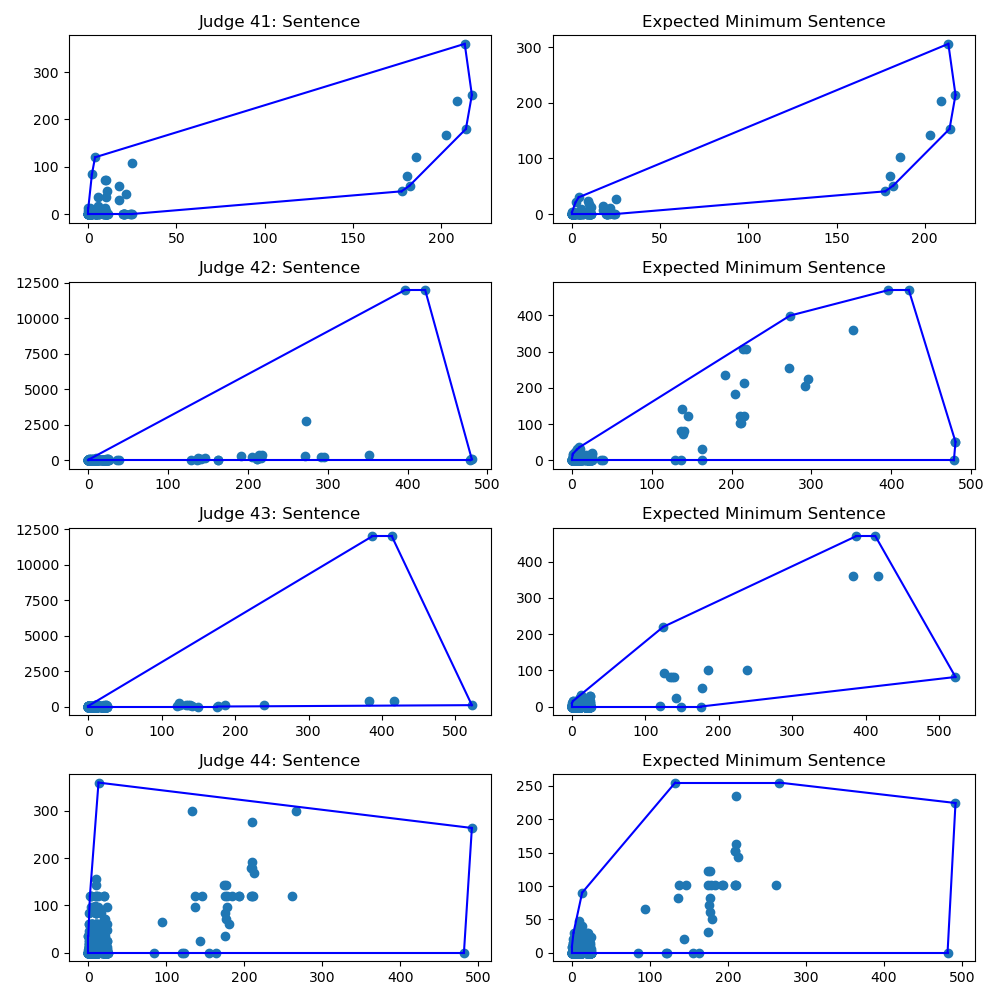
\includegraphics[width=0.9\textwidth]{../../../output/figures/Exploration/judge_convex_hulls_10.png}
  \end{figure}

  \begin{figure}[H]
    \centering
    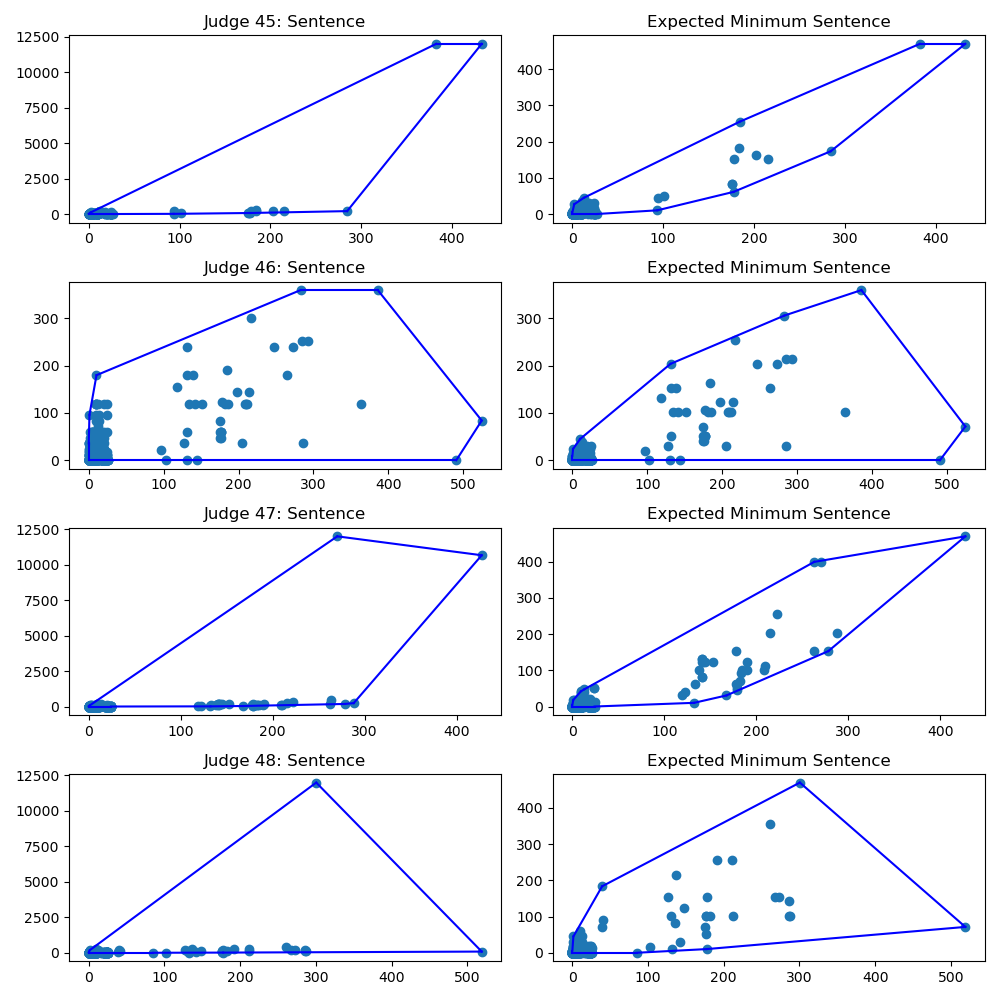
\includegraphics[width=0.9\textwidth]{../../../output/figures/Exploration/judge_convex_hulls_11.png}
  \end{figure}

  \begin{figure}[H]
    \centering
    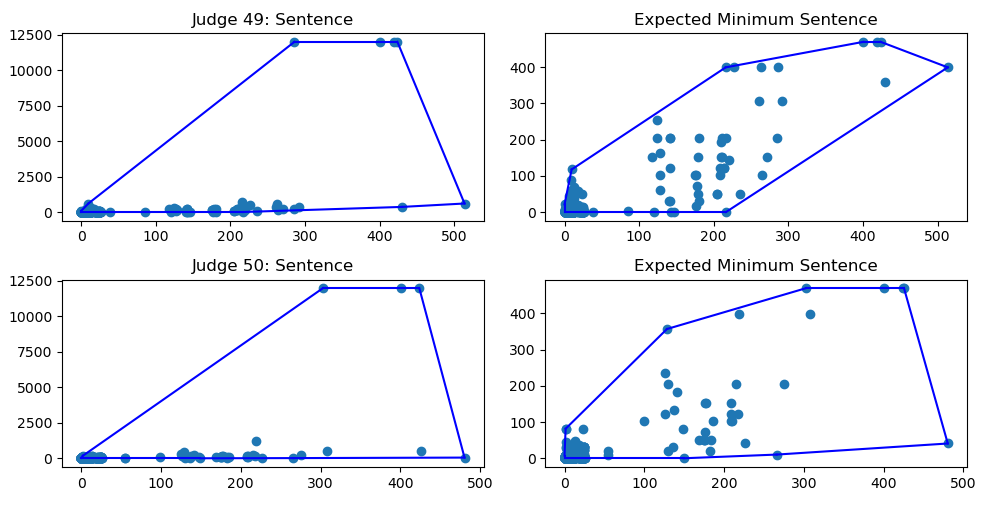
\includegraphics[width=0.9\textwidth]{../../../output/figures/Exploration/judge_convex_hulls_12.png}
  \end{figure}

\section{Distribution of pleas per day by work type}
  These are the distributions of number of pleas per day by work type. They are conditional on there being at least one sentencing event on that day. It's kind of hard to tell zeros apart from small numbers in some of the histograms, so I'm including a table with the number of days with zero pleas for each work type.

  \begin{table}[H]
    \centering
    \caption{Number of days with zero pleas by work type}
    \begin{tabular}{lr}
    WorkType &  N \\
    \hline
          CP &  1 \\
    CPNJ/PCR &  1 \\
    Disagree &  8 \\
          GS & 72 \\
       GS CC &  2 \\
    GS CP CC &  3 \\
     GS(SGJ) &  2 \\
    \hline \\
    \end{tabular}
  \end{table}


  \begin{figure}[H]
    \centering
    \caption{Histogram of pleas by work type}
    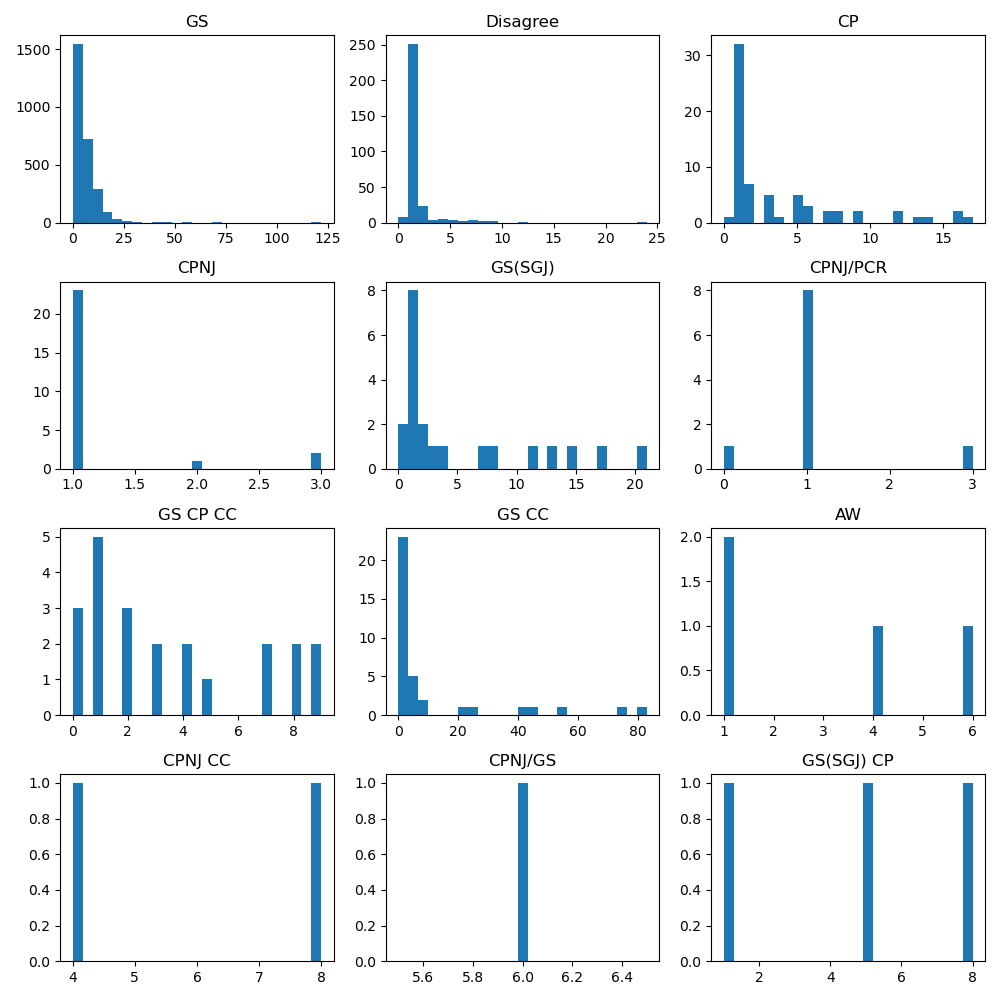
\includegraphics[width=0.85\textwidth]{../../../output/figures/Exploration/plea_by_work_type_hist.png}
  \end{figure}

\section{Trials by Resident vs Non-Resident Judges by County}
  To determine each judge's home county, I used Rhys's home circuit assignments to determine each judge's home circuit. For those judges that had a home circuit, I made their home county the county to which they are assigned to the most days according to the calendar data. In the histograms below, the blue bars are the number of trials heard by a non-resident judge, and the red bars are the number of trials heard by a resident judge.  Overall, it looks like it is common for non-resident judges to hear trials in each county. 
    \begin{figure}[H]
      \centering
      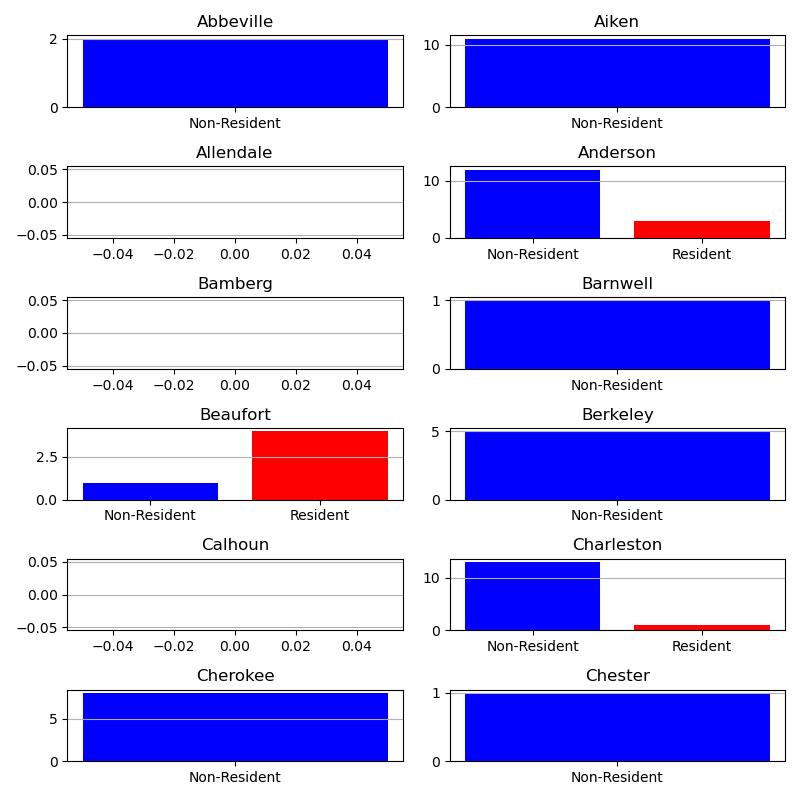
\includegraphics[width=0.9\textwidth]{../../../output/figures/Exploration/county_trial_hist_0.png}
    \end{figure}

    \begin{figure}[H]
      \centering
      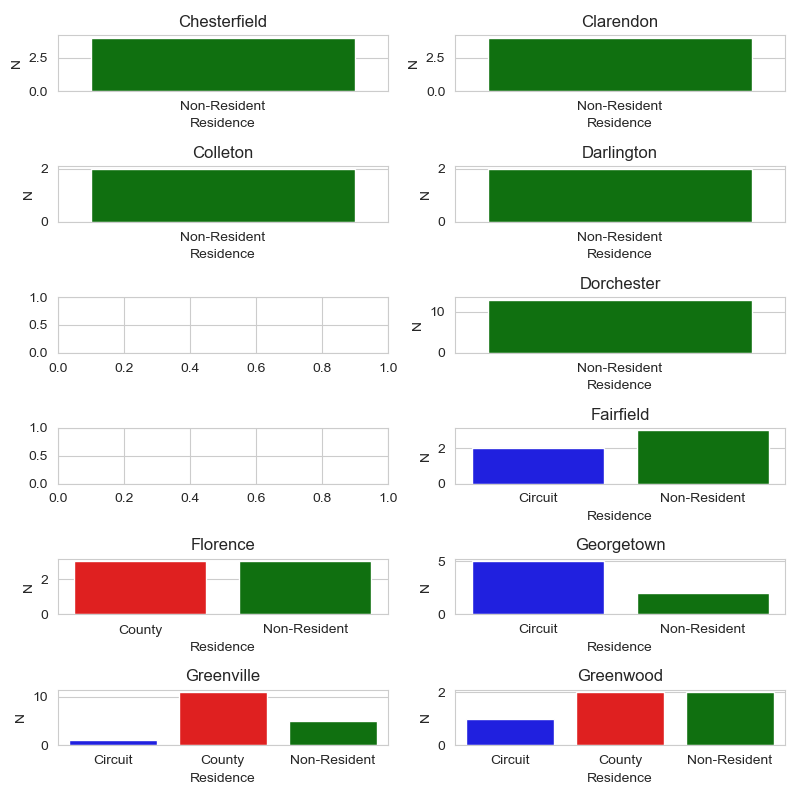
\includegraphics[width=0.9\textwidth]{../../../output/figures/Exploration/county_trial_hist_1.png}
    \end{figure}

    \begin{figure}[H]
      \centering
      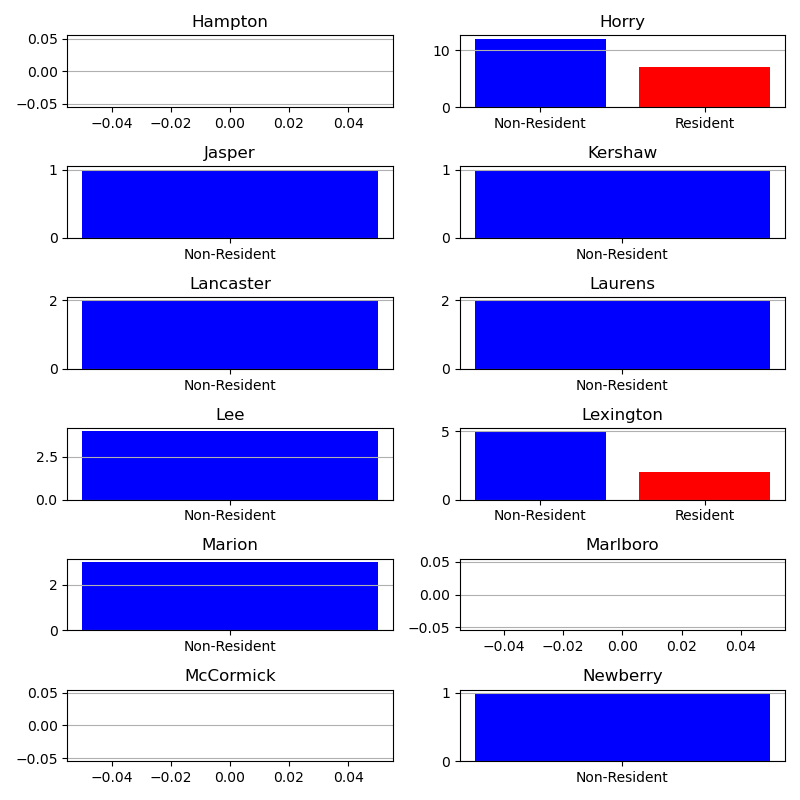
\includegraphics[width=0.9\textwidth]{../../../output/figures/Exploration/county_trial_hist_2.png}
    \end{figure}

    \begin{figure}[H]
      \centering
      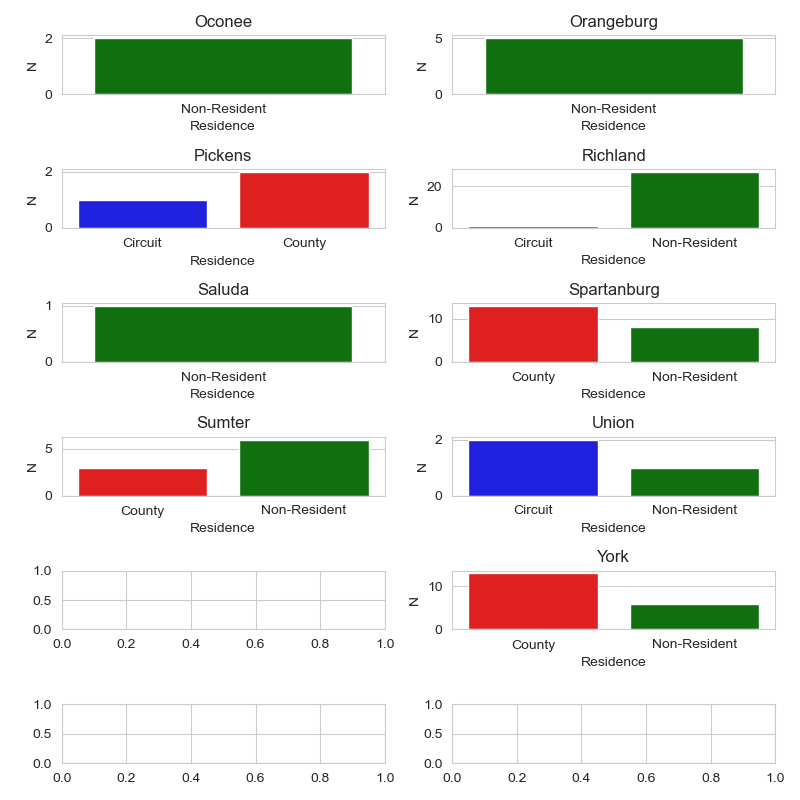
\includegraphics[width=0.9\textwidth]{../../../output/figures/Exploration/county_trial_hist_3.png}
    \end{figure}

\section{Sentencing events with missing dates}
  We will deal with trials with missing dates in the following way. Suppose judge $j$ has $m$ sentencing events with missing dates in county $c$. We first use the calendar data to determine what days judge $j$ was scheduled to be in county $c$. Let $n_{jc}$ be the number of days that judge $j$ was scheduled to be in county $c$ and let $D_{jc}$ be the set of all days in which judge $j$ was scheduled to be in county $c$. For each day $d \in D_{jc}$, we would increase the day's event count by $\frac{m}{n_{jc}}$. \textbf{Note:} I think it might be a good idea to restrict $D_{jc}$ and $n_{jc}$ to be the set/number of days in which the judge processed at least one sentencing event, otherwise, we will probably end up with a lot of days with just $1/n_{jc}$ pleas sentenced, which would be excluded from our capacity calculations because we currently exclude days with less than 1 sentencing event. However, this would assume that if a plea is processed at all, it is more likely that it was processed on a day in which other pleas were also processed. We should probably try both ways.

\section{Trial Scheduling in the Simulation}
  We first describe a method to assign a set of judges to a set of counties for T time periods. The time periods here are discrete and we think of them as weeks. We describe how the assignment would work for each individual week, but in practice all the assignments would be determined before running the rest of the simulation. Since there are 50 judges and 46 counties, in each period we would randomly draw, without replacement, 46 judges from the list of 50. Then, each of the selected judges will stay in his "home" county with probability $\eta$ and with probability $1-\eta$ he will be assigned to another county. We refer to judges that don't stay in their home county in a specific week as "rotating judges", and we refer to counties whose home judge will be rotating as "rotating counties". We assign rotating judges to rotating counties as follows: we randomly shuffle the rotating judges and the rotating counties are sorted alphabetically. So the rotating judge in the first position after shuffling would be assigned to county A, the second to County B, and so on.

  We would schedule trials in the following way. First, for each county, we would randomly select the trial dates. Then, in each time period, we would randomly assign judges to counties as described above, if a judge lands on a county on a day in which a trial is scheduled in that county, then the judge would stay there for 2 weeks. As a result, when assigning judges and counties for the next period, the county and the judge would be removed from the list of available counties/judges. In other words, the assignment for that judge and county would already be determined for the next week as well. We could then assign the remaining judges/counties using the original method.

\end{document}
